We document here the decisions taken to obtain the small image patches $x$ and its respective labels $y$ from the chosen databases.

\paragraph{Image dimensions}
We use square image patches because they are common in practice and simplify data augmentation. To define the size we have to consider two aspects: keeping a manageable input size for the network (in pixels) and capturing the entire lesion in the image patch (in mm).

The smallest microcalcification worth considering could be as small as 0.16 mm~\cite{Lo1998}, thus the spatial resolution should be at most 0.16 mm. The standard definition of a cluster of microcalcifications is of 5 or more inside a 1 $cm^2$ area~\cite{Sickles2013}, thus the entire image patch should cover at least a 1 $cm^2$ area. Using a spatial resolution of 0.16 mm and an image size of $64 \times 64$ pixels we cover an area of 1.024 cm $\times$ 1.024 cm = $\sim$1.05 $cm^2$.
% Pixel size .15625 mm i get a 10 mm2 area

Mass sizes (length of the long axis) vary from 5 mm to 20 mm~\cite{Sahiner1996}~\footnote{Bigger masses are easily detectable by touch and thus less important for our purposes.} There is not really any restriction on spatial resolution other than it being good enough to capture texture information. Using a spatial resolution of 0.32 mm and an image size of $64 \times 64$ pixels we cover an area of 2.048 cm $\times$ 2.048 cm = $\sim$4.2 $cm^2$.
% pixel size .3125 equals area 20 mm
%pixel size 0.39 equals area 25 mm
% pixel size .4 mm equals ara 25.6 mm (exactly the size in Sahiner1996)

Although we use the same input size ($64 \times 64$) for microcalcifications and masses they do not cover the same area in the mammogram. We need to use two different sizes because if we preserve the spatial resolution of 0.16 mm, the 1 $cm^2$ area would not be able to contain the entire mass meanwhile if we use a spatial resolution of 0.32 mm, some microcalcifications will dissapear and the 4 $cm^2$ area would have way too much noise compared to the size of the cluster of microcalcifications.

The low spatial resolution (big pixel sizes), however, reduces the quality of the input images. An alternative could be to use $127 \times 127$ image patches with 0.08 mm and 0.16 mm pixel sizes for microcalcifications and masses, respectively, but using a bigger filter on the first convolutional layer, for instance, a $5 \times 5$ filter with stride 2 and padding 2. This allows us to have bigger input images with a negligible increase in number of parameters. Whether the results improve or not is not clear at this point.
% The image quality is quite bad, but it's the best we can do. Going to 128 will be good if I can get some more data.

%An alternative is to use a $128 \times 128$ pixels image patch with 0.16 mm, this will result on the same 4 $cm^2$ area needed for masses with the spatial resolution needed for microcalcifications allowing us to train a single network for both kinds of lesions. Nonetheless, this has some critical flaws: the number of learnable parameters will almost double, the GPU may run into memory bottlenecks because of the increased number of parameters and unnnecesary details (noise) will be included in the image.

%Resizing

\paragraph{Cropping}
To obtain the image patches from the entire mammogram we slide a square window across the mammogram similar to the way a convolutional filter moves accross an image and store the image patch directly beneath it. This generates a big number of small patches from each mammogram and takes advantage of the translational invariance of our data, i.e., a breast mass will continue to be a breast mass no matter its position in the image patch.

An alternative is to sample the desired number of image patches at random positions from the mammograms.

\paragraph{Stride}
For input sizes of $64\times 64$ we chose a stride of 6 pixels which represents 6 $\times$ 0.16 = 0.96 mm for the microcalcifications case and 6 $\times$ 0.32 = 1.92 mm for masses. This is midway between a minimum stride of 1 which produces many image patches with maximum overlapping and 64 which produces fewer patches with no overlapping. We use a rather small stride to have a lesion appear in various image patches (although in a slightly different place in each one) and to produce a good number of patches from the original image. We use no padding.

When sliding the window starting from the upper left corner of the original image it is possible that due to a dimension mismatch pixels in the rightmost and bottom strips do not appear in any image patch, this is not a problem given that the lost strips are very thin ($\leq$ 0.8 mm for microcalcifications or  $\leq$ 1.6 mm for masses) and they are normally a black background.

\paragraph{Background}
Mammograms capture images of the breast against a black background which covers a good part of the mammogram. We delete any image patch which is 30\% or more black. No important information is lost in this process because the same part of the breast which appears in a deleted patch also appears on other image patches with less black background. A remaining question is how will the trained convolutional network react when presented with an all black input, for example, when slided across the background of a test mammogram. In practice, however, this is not relevant because it is clear that no lesion could occur outside the breast. 

An alternative is to preserve all images and let the network learn that black images are negative examples but this seems rather wasteful.

\paragraph{Assigning labels}
Once each image patch is obtained we need to assign labels to it. All image patches are initially labelled as negative (or no lesion) and only those where a lesion is present are labelled as positive. There are many ways to define the presence of a lesion in an image: (1) if a percentage of the lesion, say 70\% or more, appears in the image, (2) if a percentage of the image is covered by the lesion and (3) if a part of the lesion appears in the middle of the image.

We have chosen the last option to define the presence of a lesion because of three reasons: it is simple to implement, it somehow includes the other methods given that when a lesion appears on the middle of the image patch the rest of it will probably also appear on that patch and finally it encourages the convolutional network to output true only when the lesion appears in the center of the patch but not anywhere else which may give us more granular results when using it on the entire mammogram. The downside is that when a lesion is found on the outside of the image patch (in a corner, for example) it will be labelled as a negative example in the training set and may difficult the learning because even though the lesion is there we are training the network to answer negatively; if this effect actually occurs is not clear. \cite{Ciresan2013} uses this method to label its image patches.

Using the first or second option is a viable alternative although they come with their own caveats, for instance, it could be hard to calculate the area of irregular objects or the lesion could be so big that even covering the the entire image patch area it would still not account for 70\%.

\paragraph{Label information}
We will use the type of lession (mass, clustered microcalcifications or normal) and the malignancy (bening, malignant or nothing) to train our networks. 

Databases normally offer adittional information such as age of the patient, breast density, family clinical history, assesment of the subtlety and malignancy of the lesion, etc. This information could be used as complementary features before classification or as labels for the network. In this stage we use only the mammograms with the labels stated above (binary classification).

\paragraph{Image enhancement}
In theory we want to perform classification on the raw images (without any preprocessing) so we store the raw image patches and their labels as the base training set and perform any image enhancements during training whenever possible. There is a set of simple contrast adjustments that could be applied: normalization assigns 0 to the minimum gray value in the image and 255 (or the maximum available value) to the maximum gray value in the image and stretches the rest of the values linearly, background reduction plus normalization is similar except that all values below a given threshold (the mean of all pixel values in the image) are mapped to zero and the rest is normalized effectively reducing all small variations in the background to black and histogram equalization which tries to distribute the gray values evenly on the histogram of the image. An example of each method is shown in Fig.~\ref{fig:PreprocessingTechniques}.
\begin{figure}[h!]
	\centering
	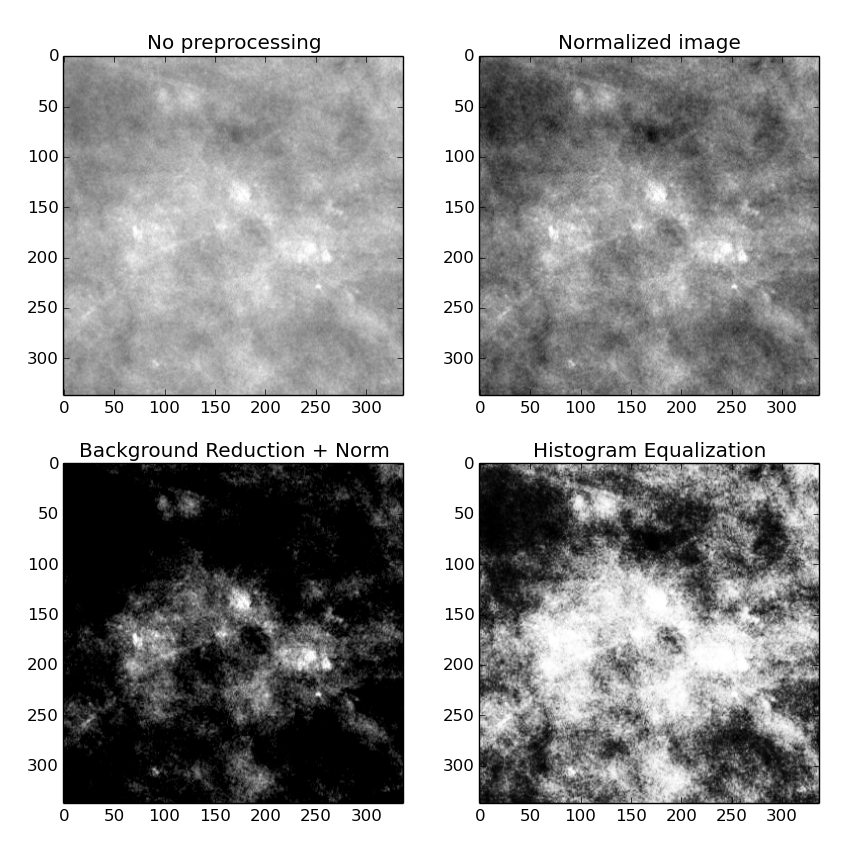
\includegraphics [width = 0.75\textwidth]{plots/mcDiffPreprocessings.png}
	\caption[Example of constrast adjustment techniques]{Example of simple contrast adjustment techniques applied to an image with a cluster of microcalcifications. Normalization takes the range of gray values and stretchs it up to linearly cover the entire range available. Background reduction assigns 0 to every pixel below the mean of the pixel values and applies normalization. Histogram equalization distributes the gray values more evenly in the histogram of the picture.}
	\label{fig:PreprocessingTechniques}
\end{figure}

We use background reduction plus normalization because it increases the signal to noise ratio, i.e., highlights lesions over normal breast tissue. On the downside, it also highlights dense structures (which could increase false positives) and may destroy important texture information by blending it with the background; using normalization only could produce better results. Unpreprocessed images seem too noisy and histogram equalization is too destructive for our purposes.

% After enhancement, we could delete those patches who are mostly black as specified above but we run the risk of deleting important info, because sometimes the white spaces are going to be small say microcalcifications but very important.

\paragraph{Data augmentation}
We augment each enhanced image by using 4 rotations (at 0°, 90°, 180° and 270°) of both the original image and a horizontally flipped version of it, thus we increase our data set by a factor of 8. Both rotations and reflections preserve the original label. In principle it is not neccesary to store the augmented images because they can be easily generated during training but if the disk space is not prohibitive explicitly storing them simplifies training.
%Does it affect to present all different augmentations of the same image in one batch rather than in different batches?

TODO: Is feature normalization needed? It does puts everything on -1 to 1 range (instead of 0-256, 0-2048, etc.). if it doesn't affect the results better do it

\paragraph{Resizing}
We have to resize the images to achieve the desired pixel size (either 0.16 mm or 0.32 mm). there is acouple of important decisions to take: the type of interpolation, which after some previous experiments prove not to be so important so we choose the recommentded by the PILLOw docs LANCZOS as implemented in there.

Enhancements are executed on each oimage patch, 
and wether we will resize the image patch and apply the enhancements on the smaller image or wether ew e will first apply the enahencment onteh big image patch and then reduce it. the difference may not be big. After some previosu experiments both proved not ot be very important so we chosse LANCzos inteprolation as impolemented in the PILLOw image python park, and the other doesn't change.
on the big image patch on 0.05 mm resolution and then resize oit or first resize it . A view of both is next. 


% Store the images one by one, a loooot of files maybe end in .patch or as a single 3-dimensional matrix for each picture ended in .patch
